% ============================================================
\chapter{Introduction to Operations Research}
\label{ch:introduction}
% ============================================================

During World War II, the Royal Air Force faced a desperate logistics
problem: how to deploy coastal radar stations to detect enemy bombers with a
limited number of installations. A group of scientists --- physicists,
mathematicians, biologists --- was assembled to analyze the problem
\emph{operationally}, using data, models, and quantitative methods. They
called their discipline ``operational research,'' and the results were
spectacular: losses dropped, efficiency soared. After the war, these methods
migrated to industry, transportation, healthcare, and finance, becoming what
we now call \emph{operations research}.

This chapter outlines the discipline: its origins, its methodology, and the
major classes of problems it seeks to solve.

% ------------------------------------------------------------
\section{What is Operations Research?}
% ------------------------------------------------------------

Let us begin by defining the subject of our study precisely.

\begin{definition}[Operations Research]
\textbf{Operations Research} (OR) is the application of scientific methods
--- mathematical, statistical, and computational --- to decision-making in
complex systems.  Its goal is to determine the best allocation of limited
resources to achieve a given objective.
\end{definition}

OR is distinguished from other branches of applied mathematics by its focus
on \emph{modelling} real-world problems and its constant concern with
providing \emph{implementable} solutions.

\begin{remark}
The term ``Operations Research'' originated in the British military during
World War~II, where ``operations'' referred to military operations.  The
discipline is also known as \textit{Management Science} or
\textit{Decision Science} in some contexts.
\end{remark}

\section{A brief history}

\subsection{Military origins (1937--1945)}

The roots of OR trace back to \textbf{Leonid Kantorovich}'s 1937 work on
optimizing production in Soviet industry.  However, the discipline truly
blossomed during World War~II:

\begin{itemize}
  \item In \textbf{1940}, physicist Patrick Blackett led
        \textit{Blackett's Circus}, an interdisciplinary team tasked with
        optimizing radar deployment and convoy sizes.
  \item In the United States, similar teams worked on bombing strategies
        and Pacific logistics.
\end{itemize}

\subsection{The foundational era (1947--1960)}

\begin{itemize}
  \item \textbf{1947}: George \textbf{Dantzig} invents the \textbf{simplex
        method} for solving linear programs.
  \item \textbf{1951}: Harold \textbf{Kuhn} and Albert \textbf{Tucker}
        formalize optimality conditions for nonlinear programming (KKT
        conditions).
  \item \textbf{1956}: Lester \textbf{Ford} and Delbert \textbf{Fulkerson}
        publish the maximum-flow algorithm.
  \item \textbf{1958}: Ralph \textbf{Gomory} introduces cutting planes for
        integer programming.
  \item \textbf{1960}: Ailsa \textbf{Land} and Alison \textbf{Doig}
        formalize \textbf{branch-and-bound}.
\end{itemize}

\subsection{Modern developments}

\begin{itemize}
  \item \textbf{1979}: Leonid \textbf{Khachiyan} proves that linear
        programming is solvable in polynomial time (ellipsoid method).
  \item \textbf{1984}: Narendra \textbf{Karmarkar} publishes the
        interior-point method, competitive with the simplex in practice.
  \item \textbf{2000s--2020s}: Modern solvers (CPLEX, Gurobi, CBC) solve
        problems with millions of variables routinely.
\end{itemize}

\section{Application domains}

OR is used across a wide range of sectors:

\begin{center}
\renewcommand{\arraystretch}{1.2}
\begin{tabular}{ll}
  \toprule
  \textbf{Sector} & \textbf{Example problems} \\
  \midrule
  Logistics & Vehicle routing, inventory management \\
  Manufacturing & Scheduling, lot sizing \\
  Finance & Portfolio optimization, risk management \\
  Transportation & Network design, bus/train timetabling \\
  Telecommunications & Routing, frequency assignment \\
  Healthcare & Operating room scheduling, bed management \\
  Energy & Unit commitment, power grid management \\
  Aviation & Revenue management, gate assignment \\
  \bottomrule
\end{tabular}
\end{center}

\section{The OR methodology}

The general OR approach follows a six-step cycle:

\begin{enumerate}
  \item \textbf{Problem definition}: identify the objective, the
        decision-makers, and operational constraints.
  \item \textbf{Data collection}: model parameters, costs, capacities,
        demands.
  \item \textbf{Model formulation}: translate the problem into mathematical
        terms (variables, objective, constraints).
  \item \textbf{Solution}: apply an algorithm or solver.
  \item \textbf{Validation}: verify the model's consistency and the
        solution's relevance.
  \item \textbf{Implementation}: deploy the solution and monitor its
        performance.
\end{enumerate}

\begin{intuition}[title=\textbf{Modelling means simplifying}]
A model is never an exact representation of reality.  The art of modelling
lies in finding the right balance between \emph{accuracy} (faithful model)
and \emph{tractability} (solvable model).
\end{intuition}

\section{Classification of optimization models}

\begin{definition}[Optimization problem]
An \textbf{optimization problem} is formulated generically as:
\[
  \min_{\mathbf{x} \in \mathcal{X}} f(\mathbf{x})
  \quad \text{subject to} \quad
  g_i(\mathbf{x}) \le 0, \; i = 1, \ldots, m,
  \qquad
  h_j(\mathbf{x}) = 0, \; j = 1, \ldots, p,
\]
where $f$ is the \textbf{objective function}, $\mathcal{X}$ the domain,
$g_i$ the \textbf{inequality constraints}, and $h_j$ the
\textbf{equality constraints}.
\end{definition}

Models are classified along several axes:

\subsection{By the nature of objective and constraints}

\begin{itemize}
  \item \textbf{Linear programming (LP)}: $f$, $g_i$, $h_j$ are all linear
        functions of $\mathbf{x}$.
  \item \textbf{Nonlinear programming (NLP)}: at least one function is
        nonlinear.
  \item \textbf{Quadratic programming}: quadratic objective with linear
        constraints.
\end{itemize}

\subsection{By the nature of variables}

\begin{itemize}
  \item \textbf{Continuous variables}: $\mathbf{x} \in \R^n$.
  \item \textbf{Integer variables}: $\mathbf{x} \in \Z^n$ (integer
        programming, IP).
  \item \textbf{Mixed variables}: some continuous, some integer (mixed-integer
        programming, MIP).
  \item \textbf{Binary variables}: $x_i \in \{0, 1\}$ (0--1 programming).
\end{itemize}

\subsection{By information availability}

\begin{itemize}
  \item \textbf{Deterministic}: all parameters are known with certainty.
  \item \textbf{Stochastic}: some parameters are random variables.
  \item \textbf{Robust}: we seek a solution that performs well across all
        possible scenarios.
\end{itemize}

\section{First modelling examples}

\begin{example}[Production problem]
A factory produces two products $P_1$ and $P_2$.  Each unit of $P_1$ yields
\$5 profit and requires 2~hours on machine~A and 1~hour on machine~B.  Each
unit of $P_2$ yields \$4 profit and requires 1~hour on machine~A and 3~hours
on machine~B.  Machine~A is available 10~hours per day, machine~B 12~hours.

\textbf{Decision variables}:
$x_1$ = units of $P_1$, $x_2$ = units of $P_2$.

\textbf{Model}:
\[
\begin{aligned}
  \max \quad & z = 5x_1 + 4x_2 \\
  \text{s.t.} \quad
    & 2x_1 + x_2 \le 10 & \text{(machine A)} \\
    & x_1 + 3x_2 \le 12  & \text{(machine B)} \\
    & x_1, x_2 \ge 0
\end{aligned}
\]
\end{example}

\begin{example}[Blending problem]
A farmer wants to prepare an animal feed mix at minimum cost.  Two
ingredients are available:

\begin{center}
\begin{tabular}{lccc}
  \toprule
  & Protein (\%/kg) & Fat (\%/kg) & Cost (\$/kg) \\
  \midrule
  Ingredient 1 & 20 & 5 & 3 \\
  Ingredient 2 & 10 & 8 & 2 \\
  \midrule
  Minimum requirement & 15 & 6 & --- \\
  \bottomrule
\end{tabular}
\end{center}

Let $x_1, x_2$ be the quantities (in kg) of the two ingredients.  The mix
must weigh 1~kg: $x_1 + x_2 = 1$.

\[
\begin{aligned}
  \min \quad & z = 3x_1 + 2x_2 \\
  \text{s.t.} \quad
    & 20x_1 + 10x_2 \ge 15 & \text{(protein)} \\
    & 5x_1 + 8x_2 \ge 6   & \text{(fat)} \\
    & x_1 + x_2 = 1 \\
    & x_1, x_2 \ge 0
\end{aligned}
\]
\end{example}

\section{Graphical solution (preview)}

For problems with two variables, we can represent the feasible set in the
plane and find the optimum graphically.

\begin{center}
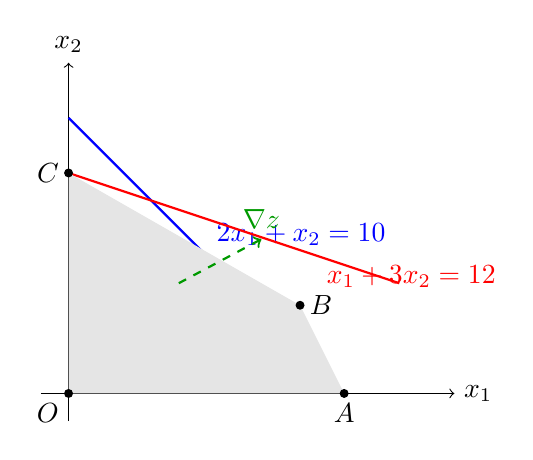
\begin{tikzpicture}[scale=0.7]
  % Axes
  \draw[->] (-0.5,0) -- (7,0) node[right] {$x_1$};
  \draw[->] (0,-0.5) -- (0,6) node[above] {$x_2$};
  % Constraint 1: 2x1 + x2 <= 10
  \draw[thick, blue] (0,5) -- (5,0)
    node[midway, above right] {$2x_1+x_2=10$};
  % Constraint 2: x1 + 3x2 <= 12
  \draw[thick, red] (0,4) -- (6,2)
    node[near end, below right] {$x_1+3x_2=12$};
  % Feasible region
  \fill[gray!20] (0,0) -- (5,0) -- (4.2,1.6) -- (0,4) -- cycle;
  % Vertices
  \filldraw (0,0) circle (2pt) node[below left] {$O$};
  \filldraw (5,0) circle (2pt) node[below] {$A$};
  \filldraw (4.2,1.6) circle (2pt) node[right] {$B$};
  \filldraw (0,4) circle (2pt) node[left] {$C$};
  % Gradient direction
  \draw[->, thick, dashed, green!60!black] (2,2) -- (3.5,2.8)
    node[above] {$\nabla z$};
\end{tikzpicture}
\end{center}

Vertex $B = (4.2, 1.6)$ maximizes $z = 5(4.2) + 4(1.6) = 27.4$.
We will confirm this result formally in Chapter~3 using the simplex method.

\section{Introduction to solvers}

\begin{codeblock}[title=\textbf{Solving with SciPy}]
\begin{minted}{python}
from scipy.optimize import linprog

# min c^T x  =>  negate for maximization
c = [-5, -4]  # max 5x1 + 4x2

# Constraints: A_ub @ x <= b_ub
A_ub = [[2, 1],   # 2x1 + x2 <= 10
        [1, 3]]   # x1 + 3x2 <= 12
b_ub = [10, 12]

# Bounds: x1, x2 >= 0
bounds = [(0, None), (0, None)]

result = linprog(c, A_ub=A_ub, b_ub=b_ub, bounds=bounds,
                 method='highs')
print(f"x* = {result.x}")
print(f"z* = {-result.fun:.2f}")
\end{minted}
\end{codeblock}

\begin{codeoutput}
x* = [4.2 1.6]
z* = 27.40
\end{codeoutput}

\begin{codeblock}[title=\textbf{Solving with PuLP}]
\begin{minted}{python}
import pulp

prob = pulp.LpProblem("Production", pulp.LpMaximize)

x1 = pulp.LpVariable("x1", lowBound=0)
x2 = pulp.LpVariable("x2", lowBound=0)

# Objective
prob += 5*x1 + 4*x2, "Profit"

# Constraints
prob += 2*x1 + x2 <= 10, "Machine_A"
prob += x1 + 3*x2 <= 12, "Machine_B"

prob.solve(pulp.PULP_CBC_CMD(msg=0))

print(f"Status: {pulp.LpStatus[prob.status]}")
print(f"x1 = {x1.varValue}, x2 = {x2.varValue}")
print(f"Profit = {pulp.value(prob.objective):.2f}")
\end{minted}
\end{codeblock}

\begin{codeoutput}
Status: Optimal
x1 = 4.2, x2 = 1.6
Profit = 27.40
\end{codeoutput}

\section{Algorithmic complexity: review}

\begin{definition}[Big-$\mathcal{O}$ notation]
An algorithm has complexity $\mathcal{O}(g(n))$ if there exist constants
$C > 0$ and $n_0$ such that the number of elementary operations is bounded
above by $C \cdot g(n)$ for all $n \ge n_0$.
\end{definition}

\begin{center}
\renewcommand{\arraystretch}{1.2}
\begin{tabular}{lll}
  \toprule
  \textbf{Class} & \textbf{Complexity} & \textbf{Example} \\
  \midrule
  $\mathcal{P}$ & Polynomial & Simplex (in practice), Dijkstra \\
  $\mathcal{NP}$ & Verifiable in polynomial time & Knapsack problem \\
  $\mathcal{NP}$-complete & As hard as any $\mathcal{NP}$ problem & TSP (decision) \\
  $\mathcal{NP}$-hard & At least as hard as $\mathcal{NP}$-complete & TSP (optimization) \\
  \bottomrule
\end{tabular}
\end{center}

\begin{warning}[title=\textbf{Simplex complexity}]
Although the simplex method has exponential worst-case complexity
(Klee-Minty examples), it is extremely efficient in practice.  Interior-point
methods offer guaranteed polynomial complexity:
$\mathcal{O}(n^{3.5} L)$ where $L$ is the input size.
\end{warning}

\section{Fundamental vocabulary}

\begin{definition}[Feasible solution]
A solution $\mathbf{x}$ is called \textbf{feasible} (or \textbf{admissible})
if it satisfies all the constraints of the problem.  The set of feasible
solutions is denoted $\mathcal{F}$ (the \textit{feasible set}).
\end{definition}

\begin{definition}[Optimal solution]
A feasible solution $\mathbf{x}^*$ is \textbf{optimal} if
$f(\mathbf{x}^*) \le f(\mathbf{x})$ for all $\mathbf{x} \in \mathcal{F}$
(in the case of minimization).
\end{definition}

\begin{definition}[Unbounded problem]
A problem is said to be \textbf{unbounded} if the objective function can take
arbitrarily small values (minimization) or large values (maximization) over
$\mathcal{F}$.
\end{definition}

\begin{definition}[Infeasible problem]
A problem is said to be \textbf{infeasible} if $\mathcal{F} = \emptyset$,
i.e., no solution satisfies all constraints simultaneously.
\end{definition}

\section{Exercises}

\begin{exercise}[$\star$ --- Modelling]
A company manufactures three products $A$, $B$, and $C$ with the following
data:

\begin{center}
\begin{tabular}{lcccc}
  \toprule
  & Machine~1 (h) & Machine~2 (h) & Machine~3 (h) & Profit (\$) \\
  \midrule
  $A$ & 1 & 2 & 1 & 10 \\
  $B$ & 2 & 1 & 3 & 15 \\
  $C$ & 1 & 1 & 2 & 12 \\
  \midrule
  Availability & 40 & 50 & 60 & \\
  \bottomrule
\end{tabular}
\end{center}

Formulate the linear program that maximizes total profit.
\end{exercise}

\begin{exercise}[$\star$ --- Graphical solution]
Solve graphically:
\[
\begin{aligned}
  \max \quad & z = 3x_1 + 2x_2 \\
  \text{s.t.} \quad
    & x_1 + x_2 \le 4 \\
    & x_1 + 3x_2 \le 6 \\
    & x_1, x_2 \ge 0
\end{aligned}
\]
\end{exercise}

\begin{exercise}[$\star\star$ --- Diet problem]
A dietitian must compose a meal at minimum cost containing at least
2000~kcal, 55~g of protein, and 800~mg of calcium.  Four foods are available:

\begin{center}
\begin{tabular}{lcccc}
  \toprule
  & kcal/100g & Protein (g/100g) & Calcium (mg/100g) & Cost (\$/100g) \\
  \midrule
  Bread & 265 & 9 & 15 & 0.30 \\
  Milk & 65 & 3.5 & 120 & 0.15 \\
  Cheese & 350 & 25 & 700 & 1.20 \\
  Apple & 52 & 0.3 & 6 & 0.40 \\
  \bottomrule
\end{tabular}
\end{center}

Formulate the corresponding LP.
\end{exercise}

\begin{exercise}[$\star\star$ --- Python code]
Implement and solve the problem from Exercise~1 using PuLP.
Verify the result with \texttt{scipy.optimize.linprog}.
\end{exercise}

\begin{exercise}[$\star\star\star$ --- Modelling with binary variables]
An investor has \$100{,}000 and must choose among 5~investment projects.
Each project $i$ requires an investment of $c_i$ and returns $r_i$.  The
investor can only invest in a project entirely (no fractions).  Moreover, if
the investor chooses project~3, then project~1 must also be selected.
Formulate this problem as an integer linear program (ILP).
\end{exercise}
